\section{Методы интерпретации}
\label{sec:Interpretation} \index{Interpretation}

\noindent\hspace{0.6cm}На сегодняшний день существует немало подходов к интерпретации прогнозов модели. Таковым может быть \textbf{конструирование похожих примеров} \cite{adversarialgenerating2}, суть которого заключается в поиске схожих примеров с точки зрения модели из тренировочных данных. Таким образом, можно понять, на какие токены модель больше всего обращала внимание для осуществления поиска. Еще одним подходом к интепретации является \textbf{изучение концепций} \cite{adversarialgenerating2}, то есть попытка выявить какие-то предрасположенности и предрассудки у модели ко входным данным. Однако в данной работе будет рассмотрена группа методов, которые тем или иным способом пытаются оценить вклад каждого отдельного токена на итоговый прогноз модели. Таким образом, данную группу методов можно охарактеризовать как \textbf{извлечение важности входных признаков}. 

\subsection{LIME}

\noindent\hspace{0.6cm}Метод \textbf{LIME} (сокращение от \textbf{Local Interpretable Model-agnostic Explanations)} представляет собой метод машинного обучения, который помогает объяснить принятие решений моделями. Он работает, создавая интерпретируемую локальную модель вокруг конкретного предсказания модели машинного обучения, и пытается оценить вклад каждого отдельного признака в итоговый прогноз \cite{optimization4}. В качестве модели, которую можно легко интерпретировать, берется \textbf{Logistic Regression}, и действительно, при нормализации признаков веса перед признаками тем больше по модулю, чем важнее сам признак. В качестве признаков LIME использует непосредственно сами слова предложения, важность которых надо извлечь (то есть для векторного представления используется модель \textbf{BOW}), а в качестве обучающей выборки LIME некоторым некоторым образом удаляет или оставляет слова в предложении, таким образом объем выборки можно довести при необходимости до $2^{n}$. LIME также учитывает не только саму структуру выборки, но и расстояние до сгенерированных объектов по некоторой метрике. Таким образом, оптимизационная задача, которую решает LIME для извлечения важности слов выглядит следующим образом:

\begin{equation*}
    \epsilon(x) = \min_{g \in G} \left\{ L(f, g, \pi_x) + \Omega(g) \right\}
\end{equation*}
\begin{equation*}
    L(f, g, \pi_x) = \sum_{z', z \in Z'} \pi_x(z)(f(z) - g(z'))^2
\end{equation*}
\begin{equation*}
    \Omega(x) = \infty\mathbbm{1}\{\|w_g\| > K\}
\end{equation*}
\begin{equation*}
    \pi_x(z) = \exp(-D(x, z)^2/\sigma^2)
\end{equation*}
где ищется Logistic Regression наилучшим образом приближающая выходы модели на конкретном тексте (L - слагаемое) и при этом не столь сложная ($\Omega$ - слагаемое), в качестве ядра $\pi_x$ используется экспоненциальное ядро.

\begin{figure}
    \centering
    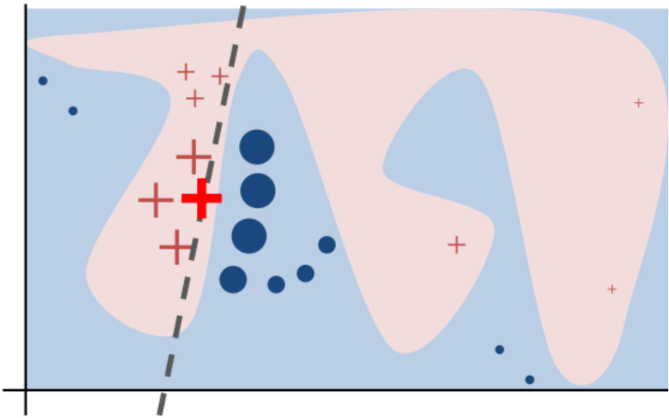
\includegraphics[width=0.5\textwidth]{pictures/lime.png}
    \caption{Иллюстрация работы метода LIME}
    \label{fig:enter-label}
\end{figure}

\noindent\hspace{0.6cm}Главная особенность lime заключается в том, что он использует исходную модель лишь как black-box, извлекая из нее лишь выходы на конкретных текстах.

\subsection{SHAP}

\noindent\hspace{0.6cm}Метод \textbf{SHAP} (расшифровывается как \textbf{SHapley Additive exPlanations}) - это способ объяснения прогнохов моделей машинного обучения, основанный на теории кооперативных игр и концепции значимости признаков. Основная идея метода SHAP заключается в том, чтобы оценить вклад каждого признака в предсказания модели, учитывая все возможные комбинации признаков \cite{optimization1}. То есть оценивается маргинальный вклад каждого отдельного признака по следующей формуле:
\begin{equation*}
    \Phi_i = \frac{1}{N}\sum_{s \in S}\frac{|S|!(K - |S| - 1)!}{K!}\{f(s \cup i) - f(s)\}
\end{equation*}
\noindent\hspace{0.6cm}При этом так как коалиции для оценки могут образовываться различными перестановками, то надо нормировать оценку на число всех возможных коалиций. Как и в методе LIME в качестве признаков выступают отдельные слова текста, которым необходимо придать определенный вес значимости
слова.

\noindent\hspace{0.6cm}Ниже проиллюстрировано схематическое устройство работы SHAP, где маргинальный вклад каждого признака “толкает” предсказание в определенную сторону, пока не получится просто предсказание модели на исходном тексте.

\begin{figure}[h]
    \centering
    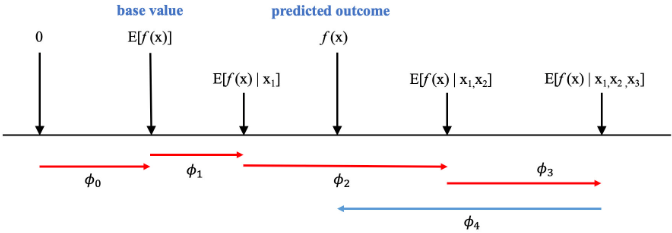
\includegraphics[width=1\textwidth, height=0.25\textheight]{pictures/shap.png}
    \caption{Иллюстрация работы метода SHAP}
    \label{fig:enter-label}
\end{figure}

\noindent\hspace{0.6cm}Как и для LIME, SHAP не требует знание о внутреннем устройстве модели и работает с ней как с black-box, извлекая лишь выходны модели на конкретном тексте. Кроме того, одной из основных особенностей метода SHAP является то, что за счет оценки важности признаков, модели можно сравнивать между собой (Если мы знаем какие признаки важны для предсказания, то та модель будет лучше, на которой SHAP придал больший вес для данного признака)

\subsection{Attention}

\noindent\hspace{0.6cm}Основная суть метода \textbf{Attention} заключается в использовании весов механизма self-attention для извлечения вклада каждого токена на каждый на $k$-ом слое transformer \cite{optimization7}. Таким образом, после прохода через модель поданных данных на выходе получается $l$ матриц весов внимания размера sequence\_len $\times$ sequence\_len, где $l$ - это количество encoder в используемой архитектуре, а sequence\_len - длина подаваемой последовательности в модель. Каждый элемент $a_{ij}^k$ такой матрицы показывает влияние $j$-ого токена на $i$-токен на $k$-ом по счету encoder. Далее данные $l$ матриц с весами внимания усредняются поэлементно и получается следующая матрица:

\[
\begin{pmatrix}
a_{11}^{res} & a_{12}^{res} & ... & a_{1seq\_len}^{res} \\
a_{21}^{res} & a_{22}^{res} & ... & a_{2seq\_len}^{res} \\
... & ... & ... & ... \\
a_{seq\_len1}^{res} & a_{seq\_len2}^{res} & ... & a_{seq\_lenseq\_len}^{res} \\
\end{pmatrix}
\]

\noindentгде $a_{ij}^{res}$ находится по следующей формуле:

\begin{equation*}
    a_{ij}^{res} = \frac{\sum_{k=1}^{l}a_{ij}^k}{l}
\end{equation*}

\noindentТаким образом, получается итоговая оценка вклада каждого токена на каждый. Для извлечения оценки важности слов на итоговый прогноз необходимо в данной полученной матрице взять 1 строку, так как в ней содержательно содержится итоговый вклад каждого токена на [CLS] токен, который используется для классификации текстов.

\subsection{ALTI}

\noindent\hspace{0.6cm}Основная идея метода \textbf{ALTI} заключается в переосмыслении значений матрицы внимания в механизме \textbf{Self-Attention} архитектуры transformer. Соответственно данный метод интерпретации работает только с \textbf{BERT}/\textbf{GPT}-подобными архитектурами. Суть данного метода заключается в декомпозиции работы механизма self-attention, в линеаризации \textbf{Layer Normalization} и перевзвешивании вклада каждого скрытого вектора \cite{optimization6}.

\noindent\hspace{0.6cm}Как уже известно: в различных архитектурах используется нормализации данных для ускорения обучения, в частности в трансформерах используется нормализация вдоль скрытого состояния каждого слова по следующей формуле:

\begin{equation*}
    LN(u) = \frac{u - \mu(u)}{\sigma(u)}\cdot\gamma + \beta
\end{equation*}

\noindentОднако можно показать, что данное преобразование можно представить в матричном виде по следующей формуле:

\begin{equation*}
    LN(u) = \frac{1}{\sigma(u)}Lu + \beta
\end{equation*}

\noindentгде матрица L представляется в следующем виде:

\[
L = \begin{array}{c c}
\begin{pmatrix}
\gamma_1 & 0 & ... & 0 \\
0 & \gamma_2 & ... & 0 \\
... & ... & ... & ... \\
0 & 0 & ... & \gamma_n \\
\end{pmatrix}
&
\begin{pmatrix}
-\frac{n - 1}{n} & -\frac{1}{n} & ... & -\frac{1}{n} \\
-\frac{1}{n} & -\frac{n - 1}{n} & ... & -\frac{1}{n} \\
... & ... & ... & ... \\
-\frac{1}{n} & -\frac{1}{n} & ... & -\frac{n - 1}{n} \\
\end{pmatrix}
\end{array}
\]

Таким образом, multi-head self-attention для поданных векторов $x_i$ можно переписать следующим образом:
\begin{equation*}
    \widehat{y_i} = LN(\widehat{x_i} + x_i)
\end{equation*}

где
\begin{equation*}
    \widehat{x_i} = W_oConcat(z^1_i, ..., z^H_i), z^h_i = \sum_{j}^{J}A^h_{i,j}W^h_{V}x_j
\end{equation*}

то есть
\begin{equation*}
    \widehat{x_i} = \sum_{h}^{H}W^h_oz^h_i + b_o
\end{equation*}

тогда получается
\begin{equation*}
    y_i = LN(\sum_{j}^{J}\sum_{h}^{H}W^h_oA^h_{i,j}W^h_Vx_j + b_o + x_i) = \sum_{j}^{J}T_i(x_j) + \frac{1}{\sigma(\widehat{x_i} + x_i)}Lb_o + \beta
\end{equation*}

при учете, что
\[
T_i(x_j) =
\begin{cases}
    \frac{1}{\sigma(\widehat{x_i} + x_i)}L\sum_{h}^{H}W^h_oA^h_{i,j}W^h_Vx_j & \text{если } i = j \\
    \frac{1}{\sigma(\widehat{x_i} + x_i)}L(\sum_{h}^{H}W^h_oA^h_{i,j}W^h_Vx_j + x_i)   & \text{если } i \neq j \\
\end{cases}
\]

\noindentТо есть показано, что влияние j-го признака на i-ый выражается через вектор
$T_i(x_j)$ на некотором $l$-ом по счету encoder, однако простая $\|*\|_2$ норма от
$T_i(x_j)$ приведет лишь к тому, что: 
\begin{enumerate}
    \item произойдет потеря информации о расположении в пространстве данного вектора
    \item если в векторе $T_i(x_j)$ присутствуют слишком большие значения, то их влияние будет доминирующим при финальном учете важности, что негативно сказывается на итоговой оценке весов слов.
\end{enumerate}
Для борьбы с данными проблемами был предложен немного иной пересчет важности вклада каждого отдельного слова по следующим формулам:
\begin{equation*}
    d_{i,j} = \|y_i - T_i(x_j)\|_1
\end{equation*}
\begin{equation*}
    c_{i,j} = \frac{\max(0, -d_{i, j} + \|y_i\|_1)}{\sum_{k}\max(0, -d_{i, j} + \|y_i\|_1)}
\end{equation*}

\begin{figure}[h]
    \centering
    \begin{minipage}{0.55\textwidth}
        \centering
        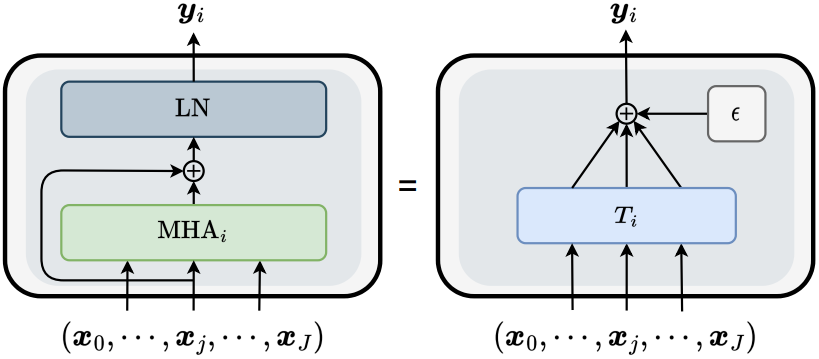
\includegraphics[width=\textwidth]{pictures/alti1.png}
        \caption{Декомпозиция ALTI}
        \label{fig:image1}
    \end{minipage}
    \begin{minipage}{0.3\textwidth}
        \centering
        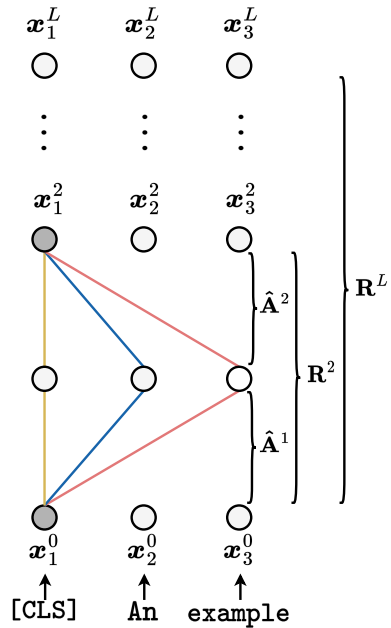
\includegraphics[width=\textwidth]{pictures/alti2.png}
        \caption{Rollout}
        \label{fig:image2}
    \end{minipage}
\end{figure}

\noindent\hspace{0.6cm}Таким образом, учитывается пространственная информация, и уходит вырожденность важности вектора в важность одного большого значения в векторе. Последняя модификация в методе ALTI - это метод \textbf{Rollout}, который позволяет отследить влияние исходного токена при подачи в трансформер на скрытое представление токена после механизма self-attention на некотором $l$-ом по счету encoder. Пусть $A$ - некоторая матрица весов важности, тогда с учетом \textbf{residual connection} вклад токена на другой токен через один encoder можно выразить как:
\begin{equation*}
    \widehat{A^l} = 0.5A^l + 0.5I
\end{equation*}
\noindentТогда для учета важности влияния исходных токенов на скрытые представления токенов после механизма self-attention на $l$-ом по счету encoder выразиться как:
\begin{equation*}
    R = \widehat{A^l}*\widehat{A^{l-1}}*...*\widehat{A^1}
\end{equation*}

\noindentТо есть матрица R будет содержать те самые обновленные веса важности каждого токена на каждый. Объединив все преобразования, в итоге получим:
\begin{equation*}
    R = \widehat{C^l}*\widehat{C^{l-1}}*...*\widehat{C^1}
\end{equation*}

\subsection{Gradient}

\noindent\hspace{0.6cm}Основная суть метода \textbf{Gradient × Input} заключается в том, что выход модели аппроксимируется по первому члену из разложения в \textbf{ряд Тейлора} \cite{optimization3}:

\begin{equation*}
    m(X^o) \approx grad(m(X^o)) * X^o
\end{equation*}

\noindentТаким образом выход приблизительно равен градиенту в точке на значение самой точки и автоматически получается оценка важности каждого отдельного признака. Но не всегда такую оценку возможно получить, так как на некоторых участках функция может быть постоянной, поэтому градиенты дадут $0$ значение. Модификацией простого метода Gradient × Input является \textbf{Integrated Gradients} \cite{optimization3}, которые учитывают изменение функции не только в конкретное точки а вдоль прямой линии между данной точкой и некоторым baseline $x^o$ по следующей формуле:

в непрерывном случае
\begin{equation*}
    IntegratedGrads_i(x) = (x_i - x^o_i) \int_{\alpha=0}^{1}\frac{\partial F(x^o + \alpha*(x - x^o))}{\partial x_i}\, d\alpha
\end{equation*}

или в дискретном случае
\begin{equation*}
    IntegratedGrads_i(x) \approx (x_i - x^o_i) * \sum_{k=1}^{m}\frac{\partial F(x^0 + \frac{k}{m} * (x - x^0))}{\partial x_i} * \frac{1}{m}
\end{equation*}

\noindent\hspace{0.6cm}Одно из главных свойств Integrated gradients заключается в том, что отслеживается изменение не только в конкретной точке, а на пути к этой точке от некоторой другой, что делает невозможным ситуацию, когда Integrated gradients были бы равны 0. Кроме того Integrated Gradients обладают важным свойством в случае когда целевая функция F (нейронная сеть) почти везде
дифференцируема (что истинно почти всегда):

\begin{equation*}
    \sum_{i=1}^{m} IntegratedGrads_i(x) = F(x) - F(x^0)
\end{equation*}

\noindentТо есть если взять baseline, при котором $F(x^o) \approx 0$, то получится разложение
значения функции F в точке на признаки с весами, равными их важности.